\documentclass{egpubl}
\usepackage{wait2021}

%\ConferencePaper      % uncomment for (final) Conference Paper

\title{Visualization of relativistic phenomena}
\author{Zoltán Simon
%\thanks{Dr. Nándor Bokor, Dr. László Szirmay-Kalos}
}

%for including postscript figures
\usepackage[dvips]{graphicx}
% \usepackage[dvips,draft]{graphicx}% replace PS figure by framed file name

\PrintedOrElectronic

% prepare for electronic version of your document
\usepackage{t1enc,dfadobe}

%Graphics include path
\graphicspath{ {./images} }
\DeclareGraphicsExtensions{.png}


% For backwards compatibility to old LaTeX type font selection.
% Uncomment if your document adheres to LaTeX2e recommendations.
\let\rm=\rmfamily    \let\sf=\sffamily    \let\tt=\ttfamily
\let\it=\itshape     \let\sl=\slshape     \let\sc=\scshape
\let\bf=\bfseries

% if the Editors-in-Chief have given you the data, you may uncomment
% the following five lines and insert it here
%
% \volume{22}   % the volume in which the issue will be published;
% \issue{3}     % the issue number of the publication
% \pStartPage{???}      % set starting page

\begin{document}

\maketitle

\begin{abstract}
Special relativity describes many phenomena, not observable in everyday life. This article presents an educational application, which helps to understand these effects. It models vision of objects travelling close to the speed of light. It visualizes length contraction, time dilatation, relativistic Doppler effect and more. It considers the path of light between the object and our eye, but it also presents an opportunity to visualize events happening simultaneously as well. It allows to switch between Lorentz and Galilean transformation, so we can compare Einstein's and Newton's model. It serves with a three-dimensional space-time diagram, on which we have a chance to further analyse the movement of objects.
\begin{classification} % according to http://www.acm.org/class/1998/
\CCScat{I.3.3}{Computer Graphics}{Visualization of relativistic phenomena}
\end{classification}

\end{abstract}

\section{Introduction}
Theory of relativity is a key part of modern physics. There are many use cases of this theory. Despite of it's importance there is very little chance for people to experience relativistic phenomena in their everyday life, thus differences between Isaac Newton's classical and Albert Einstein's modern model remain unexplored. The application described in this article offers a way to visualise the most well-known phenomena associated with special relativity. The goal of this article is to showcase the algorithmic challenges surrounding this program and introduce solutions for these problems. 


\section{Previous Work}

This article is a direct follow up of the work \cite{TDKreport}. It explains previously neglected details, e.g. implementation of Wigner-rotation. 



\section{Our proposal in detail}

%
%Visualization of relativistic phenomena content:
%

\section{Implementation of physical models}
The rules of simulation are based on Einstein's postulates~\cite{EinsteinElectrodynamics}. These suggest that
\begin{itemize}
\item an observer can not differentiate between different inertial frames of reference by taking measurements in each frame of reference.
\item the velocity of propagation of any physical effect can not exceed
the speed of light in vacuum: $c=299792458 \frac{m}{s} \sim 3 \cdot 10^8 \frac{m}{s}$.
 \end{itemize}
These two constraints do not provide sufficient tools for the programmer on their own. However, all the required formulas can be derived from these two postulates.

\subsection{Usage of the term ,,absolute frame''}
To simplify representation of world lines every event and velocity is described in the same frame of reference. In code this frame of reference is called absolute frame. This helps circumvent confusion when transforming between different observer's proper frames. Each value is stored as it is measured in absolute frame. When visualising a given value, than it gets transformed to a particular observers proper frame.

\subsection{Representation of physical bodies}
To model the journey of physical objects through space-time, it is convenient to assign a world line to each object. To be more precise, this is going to be the world line of the object's origin. For practical purposes this origin point is selected to be the same as the origin point in model space. Such world line can be stored as a set of events. Between the events we assume geodetic world lines. At this point it is necessary to note, that we also assume flat space-time. This method allows us to represent world lines consisting of few geodetic sections easily. World lines of accelerating objects appear curved in space-time diagrams. We can approximate these lines by a set of short geodetic sections. This approximation is useful, because along the small sections we can use the simple formulas of Lorentz transformation . The downside of this method is, that many calculations require iteration over the small sections. E. g. determining the age of an object without a priory information requires summing of ageing of the object along the geodetic sections. The other obvious downside of such approximation is, that the resulting world line is going to have low resolution. This is particularly noticeable, when we --as a viewer-- place ourselves in the proper frame of such accelerating object. In this case the violent jumping nature of the movement of surroundings is much more noticeable.

\section{View modes}
The application supports multiple view modes. The two main modes are the \emph{real time} three dimensional view and the \emph{diagram view}. In the \emph{real time} mode the scene is shown as regular three dimensional scene, changing over time. We can look around with the virtual camera to observe the moving objects. The shape and colour of objects gets distorted in accordance with the relativistic effects. 

In the \emph{diagram view} we can observe the world lines of objects present in the scene. This provides additional insight into the behaviour of objects. As a recent addition to the project now the user can switch to orthographic projection from the standard perspective projection. This improves the readability of the space-time diagram, and it's also useful in the \emph{real time} view.

In order to help the user spot the differences between classic and relativistic physics, there is a way to switch between Galilean \cite{KHGalilei} and Lorentz transformation. A viewer can see the incoming light from an object, thus we can only see images showing the past. This is due to the finiteness of the speed of light. The application allows to toggle between visualisation of present event and past events in accordance with the incoming light beams.

\subsection{Switching between observers}
To compare the observations in different inertial frames of reference, we can toggle between multiple observers. In this implementation observers are independent from physical objects, however it's possible to make an observer follow an object. Every observer has it's own world line. These lines are also visible in \emph{diagram view}.

When switching between frames of reference the origin of the frame also changes. The $\vec{O} =(0,0,0)$ in current proper frame gets assigned to the space coordinate vector of an event along the world line of the observer. The question is, how do we select the time component. In other words which event will be selected along the new world line. This implementation chooses the event from the new observers world line, which happened simultaneously whit the event of changing observers according to the previous observers. This method introduces a somewhat more realistic approach, however in real life still no object can travel from one event's location to an other's if these two events appear to be simultaneous. In defence of this approach in this computer simulation neither the user's perspective nor an observer is bound to a physical object.

\begin{figure}[hbp]
%\makebox[\textwidth]{\framebox[5cm]{\rule{0pt}{5cm}}}
%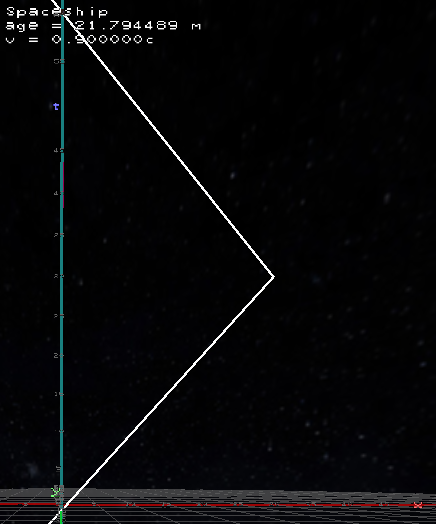
\includegraphics[scale=1]{travelingTwin}
\end{figure}






%---------------------------------------------------------------------

\section{Digitising Errors}
\label{sec:digErr}

Like most cartographic algorithms, the Douglas--Peucker algorithm does not
fully address the issue of digitising errors. When estimating truth values,
it is usually assumed that the true line (in this case the analogue line)
lies within the error band of the digitised line. This band is also known as
the Perkal epsilon band. In his review on issues relating to the accuracy of
spatial databases, Goodchild\cite{Lev90} indicated that researchers have
proposed uniform, normal and even bimodal distributions of error across this
band. This concept provides some basis for estimating the position of the
true line at locations between digitised points. Here, we are merely
concerned with the accuracy of digitised points. Whilst it is probable that
operators digitise points along high curvatures more carefully than at
intermediate positions, there is at present no sound basis for modelling the
distribution of error along the line. As in the Circular Map Accuracy
Standard, it is usual to assume a bivariate normal distribution of error when
estimating the position of the true point. In the context of line
simplification, absolute positional accuracy is less important than the
relative position of points describing the shape of features along the line.

The DoE/SDD boundary data contain some gross digitising errors. For example,
inlet X in Figure~2c does not feature on conventional Ordnance Survey
1:\,50\,000 maps of the area. The data are also not very accurate where
coastlines are convoluted. Even if we ignore these and other gross errors,
such as spikes, there will always be an element of random error in digitised
data. It is reasonable to assume that points digitised from 1:\,50\,000
source material may only be accurate to within $+/-5$ metres. This algorithm
does not lead to a substantial accumulation of rounding errors, hence the
numerical errors discussed earlier tend to be very small compared with
digitising errors.

For the purposes of our argument, it is unnecessary to undertake an
exhaustive evaluation of the consequences Douglas and Peucker have treated
overhangs and closed loops as different problems, and have used different
methods to cope with each case.

\subsection{Numerical Problems}

The FORTRAN programs by Douglas, White, and Wade use single precision REALS
when computing offsets (see results in Table~\ref{tab:calcPrec}). Whilst
double precision accuracy may be attained through the use of compiler
options, we are unsure whether previous research has been based on programs
compiled in this manner. Wade's program was so compiled for use in our
previous evaluations. Forrest stated that Ramshaw (1982) had to adopt
carefully tuned double and single precision floating point arithmetic to
compute the intersection of line segments whose end points were defined as
integers. Forrest exclaimed ``This is an object lesson to us all:
constructing geometric objects defined on a grid of points, requiring ten
bits for representation can lead to double precision floating point
arithmetic!''.

Most evaluative studies do not cite the co-ordinates in use. We do not know
whether the published test lines were in original digitiser co-ordinates or
whether they had been converted to geographic references. British National
Grid co-ordinates for the administrative boundaries of England, Scotland and
Wales (digitised by the Department of Environment (DoE) and Scottish
Development Department (SDD)) are input to one metre accuracy and require
seven decimal digits for representation if we include the northern islands of
Scotland. At the South West Universities Regional Computer Centre these
co-ordinates have been rounded to 10 metre resolution; even this requires six
decimal digits. Seamless cartographic files at continental and global scales
use much larger ranges of geographic co-ordinates.

\begin{table}[htb]
%\begin{center}
\small
\begin{tabular*}{\linewidth}%
{@{}l@{}l@{}c@{}c@{}c@{}l@{}}
\hline
Machine\,\,\, & Points &
\multicolumn{4}{@{}c}{\small Calculated squares of offset values}\\
 & & \multicolumn{2}{@{}c}{\small Single Precision}
& \multicolumn{2}{c@{}}{\small Double Precision}\\
\hline
\multicolumn{6}{@{}l}{ICL 3980} \\
& (C) & \multicolumn{2}{@{}c}{28199.351562500}
& \multicolumn{2}{c@{}}{28143.490838958}\\
 & (D) & \multicolumn{2}{@{}c}{28171.789062500}
& \multicolumn{2}{c@{}}{28143.490838961}\\
\multicolumn{6}{@{}l}{VAX 8200} \\
& (C) &\multicolumn{2}{@{}c}{28253.095703125}
&\multicolumn{2}{c@{}}{28143.490838958}\\
& (D) &\multicolumn{2}{@{}c}{28165.806640625}
&\multicolumn{2}{c@{}}{28143.490838958}\\
\multicolumn{6}{@{}l}{SEQUENT SYMMETRY}\\
& (C) &\multicolumn{2}{@{}c}{28145.100000000}
&\multicolumn{2}{c@{}}{28143.490838961}\\
& (D) &\multicolumn{2}{@{}c}{28145.100000000}
&\multicolumn{2}{c@{}}{28143.490838961}\\
\multicolumn{6}{@{}l}{SUN 3/60} \\
& (C) &\multicolumn{2}{@{}c}{28253.095703125}
&\multicolumn{2}{c@{}}{28143.490838961}\\
& (D) &\multicolumn{2}{@{}c}{28165.806640625}
&\multicolumn{2}{c@{}}{28143.490838961}\\
\hline
\\
\multicolumn{6}{@{}l}{\textsc{Notes}}\\[5pt]
\multicolumn{6}{@{}p{\linewidth}@{}}
{\emph{Offsets of points C and D from the anchor-floor line
A--B as calculated using Wade's program. Points A, B, C and D are shown in
Figure 5. The British National Grid coordinates (in metres) of the points
are as follows:}}\\[9pt]
\hline
Point A & \multicolumn{2}{l}{238040\,\, (x1)}  &
\multicolumn{2}{l}{205470\,\, (y1)}
&  \multicolumn{1}{c}{ANCHOR}\\
Point B  & \multicolumn{2}{l}{237890\,\, (x2)}
& \multicolumn{2}{l}{205040\,\, (y2)}
& \multicolumn{1}{c}{FLOATER}\\
Point C & \multicolumn{2}{l}{237810\,\, (x3)} &
\multicolumn{2}{l}{205320\,\, (y3)} & \\
Point d  & \multicolumn{2}{l}{238120\,\, (x3)} &
\multicolumn{2}{l}{205190\,\, (y3)} & \\
\hline\\
\multicolumn{6}{@{}p\linewidth@{}}{\emph{Note that the
above co-ordinates may be used in conjunction
with the expression presented in section 3.2.2a to check the tabulated
results.}}
\end{tabular*}
%\end{center}
\caption{\label{tab:calcPrec} The Precision of Calculations}
\end{table}

A limited number of papers actually described improved for new algorithms or
methods for visual\-ization\cite{Lev90,PorDuf84,RonRos96}. This may be caused
by the complexity of the environment in which a method is used; issues of
system architecture, user interface, data handling, etc. must be dealt with
before a new presentation technique can show its full advantage. But even so,
we think the field can use more contributions of this type.

There was also a discussion session on the merits of animation and special
effects (such as sound) to support visualization. For example, in the area of
flow visualization, it is quite common to use animation, and techniques for
video registration have been developed.

\section{Issues in Visualization}

Scientific visualization is an interdisciplinary field, which can only
flourish when computer graphics experts cooperate with specialists from
application areas, and providers of computing, visualization, and data
management facilities. Therefore, it is essential that all of these
viewpoints are represented in research projects and also in meetings such as
this workshop. It is not enough that suitable display algorithms, data
structures, or user interfaces be developed, but also that these be
integrated in usable systems and evaluated by expert users. This complex
environment, and the complex systems it requires, call for a common language
between different parties involved, and therefore \emph{a reference model}, or
an abstract description summarizing the entire process of data visualization,
is needed.

At the Delft workshop, an attempt was made to continue the meetings of
sub-groups as started in Clamart\cite{yll}, but it appeared that a useful
description of sub-areas or sub-problems should be based on a stable
conceptual framework. Except for the flow visualization group, the subgroup
definitions were abandoned, and instead it was decided to concentrate on
design of an initial reference model; a first attempt is currently being
undertaken by Lesley Carpenter and Michel Grave. At the same time, the
separate flow visualization sub-group (chaired by Hans-Georg Pagendarm)
agreed to design a general model of the flow visualization process! In
addition, arrangements were made for the exchange of test data sets for
system evaluation, and the exchange of information on and experience with
visualization software.

Special discussion sessions were held about the practice the ``circle-brush''
algorithm. In this algorithm a solid disk is assumed to move along a
trajectory in $R^2$. This trajectory is then scan-converted into the raster
plane. and experience of the Stardent AVS system, and about general
evaluation methods for visualization software. There is an obvious need to
share experience or even make a formal (comparative) evaluation of systems,
but this is also hampered by lack of a common framework, and also by the
continuing development of visualization systems.

Interactive visualization was also an interesting subject for discussion,
which yielded a lively debate\cite{yll}. In a session about visualization
facilities, it was suggested from experience that large research institutes
might well have to employ specialized `visualization experts', to bridge the
gap between complex numerical simulations and sophisticated visualization
facilities.


\section{Results}
\label{sec:results}

This section only refers a table with some numerical results (see
Table~\ref{tab:calcPrec}). \\
Non-sense text follows text text text text text text text text text text text
text text text text text text text text text text text text text text text
text text text text text text text text text text text text text text text
text text text text text text text text text text text text text text text
text text text text text text text text text text text text text text text
text texttext text text text text.


\section{Conclusions}
\label{sec:concl}

Here are conclusions and possible extensions. As shown by the results
reported in Section~\ref{sec:results} and in Figure~\ref{fig:ex3} (see color
plates), conclusions conclusions conclusions conclusions conclusions
conclusions conclusions conclusions conclusions conclusions conclusions
conclusions conclusions conclusions conclusions conclusions conclusions
conclusions conclusions conclusions. Conclusions conclusions conclusions
conclusions conclusions conclusions conclusions conclusions conclusions
conclusions conclusions conclusions conclusions conclusions conclusions
conclusions conclusions conclusions conclusions conclusions conclusions
conclusions conclusions conclusions.


\section*{Acknowledgements}

Introduce here, if you would....


\begin{thebibliography}{1}


\bibitem{TDKreport} Zoltán Simon.
\newblock Visualization of relativistic phenomena.
In \emph{Villamosmérnöki és Informatikai Kar 2021. évi TDK}, Szoftver, November 2021.

\bibitem{EinsteinElectrodynamics} Albert Einstein.
\newblock On the Electrodynamics of Moving Bodies.
In \emph{Annalen der Physik}, \textbf{17}:891, June 1905.

\bibitem{AERelativity} Albert Einstein.
\newblock \emph{Relativity: The Special and General Theory}.
Henry Holt and company, 1920.

\bibitem{KHGalilei} Knudsen J.M., Hjorth P.G. The Galilei Transformation.
In \emph{Elements of Newtonian Mechanics}. Advanced Texts in Physics. Springer, Berlin, Heidelberg, 2000.

\bibitem{BRGPS} Buenker, Robert J.
\newblock The Global Positioning System and the Lorentz Transformation.
In \emph{Apeiron: Studies in Infinite Nature}, 15.3, 2008.



% Template items:

\bibitem{yll} Y. Le Lous,
``Report on the First Eurographics Workshop on Visualization in
Scientific Computing'', \emph{Computer Graphics Forum\/}
\textbf{9}(4), pp. 371--372 (December 1990).

\bibitem{FolDamFeiHug.etal93}
J. Foley, A. van Dam, S. Feiner, J. Hugues, and R. Phillips.
\newblock \emph{Introduction to Computer Graphics}.
\newblock Addison Wesley, 1993.

\bibitem{PosFel89}
K.Ch. Posch and D.W. Fellner.
\newblock The Circle-Brush Algorithm.
\newblock \emph{Transactions on Graphics}, \textbf{18}(1):1--24, 1989.

\bibitem{FolHagNie93}
T.A. Foley, H.~Hagen, and G.M. Nielson.
\newblock Visualizing and modeling unstructured data.
\newblock \emph{The Visual Computer}, (9):439--449, 1993.

\bibitem{Lev90}
M.~Levoy.
\newblock Efficient ray tracing of volume data.
\newblock \emph{ACM Transactions on Graphics},
          \textbf{9}(3):245--261, July 1990.

\bibitem{PorDuf84}
T.~Porter and T.~Duff.
\newblock Compositing digital images.
\newblock \emph{ACM Computer Graphics (Proc. of SIGGRAPH '84)},
          \textbf{18}:253--259, 1984.

\bibitem{RonRos96}
R.~Ronfard and J.~Rossignac.
\newblock Full-range approximation of triangulated polyhedra.
\newblock \emph{Computer Graphics Forum (Eurographics'96 Proc.)},
          \textbf{15}(3):67--76, 1996.

\end{thebibliography}

\end{document}
%%%%%%%%%%%%%%%%%%%%%% end of VisualizationOfRelativisticPhenomena.tex %%%%%%%%%%%%%%%%%%%%%%
